\documentclass{lecturenotes}

\renewcommand{\vecka}{6}
\newcommand{\tema}{Vektorer}

\setbeamertemplate{footline}[frame number]
\title[Föreläsningsanteckningar EDA016, 2015]{EDA016 Programmeringsteknik för D}
\subtitle{Läsvecka \vecka: \tema}
\author{Björn Regnell}
\institute{Datavetenskap, LTH}
\date{Lp1-2, HT 2015}
 
\begin{document}

\frame{\titlepage}
\setnextsection{\vecka}
\section[Vecka \vecka: \tema]{\tema}
\frame{\tableofcontents}

%%%%%%%%%%%%%%%%%%%%%%%%%%%%%%%%%%%%%%

\subsection{Att göra denna vecka}
\begin{Slide}{Att göra i Vecka \vecka: Förstå vektorer (eng. Arrays)}
\begin{enumerate}
\item Läs följande kapitel i kursboken: 8 \\  
Begrepp: element, vektor, Array, allokering, indexering
\item Gör övning 6: vektor, registrering
\item Träffas i samarbetsgrupper och hjälp varandra 
\item Gör Lab 5: Gissa Tal \\ Om den är för lätt: bygg ut den, gärna med grafik i SimpleWindow
\end{enumerate}
\end{Slide}

\subsection{Vektorer}
% Ide till övning: medelvärde (heltal i vektor) med tillämpning på bonusuträkning. 
%% Quest: Hur ska vi göra med decimaler? (Reellt beslut i kursen krävs då detta ej är def. i kursprog)


\begin{Slide}{Datastrukturer}
En datastruktur:

\begin{itemize}
\item kan innehålla många element,
\item har \emph{ett} namn,
\item och man kan komma åt de enskilda elementen.
\end{itemize}

Man kan organisera elementen på olika sätt, till exempel som listor, träd eller grafer:

\begin{center}
\includegraphics[width=8cm]{fkap8/lista.pdf}\\
\vspace{5mm}
\includegraphics[width=4cm]{fkap8/trad.pdf}
\hspace{5mm}
\includegraphics[width=4cm]{fkap8/graf.pdf}
\end{center}
\end{Slide} 
%
%\begin{frame}[fragile=singleslide]
%\frametitle{Vektorer}
%\begin{center}
%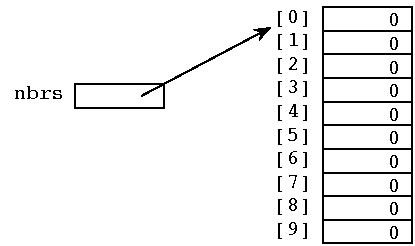
\includegraphics[scale=0.9]{fkap8/vektorbild1.pdf}
%\end{center}
%\begin{Code}
%int[] nbrs = new int[10]; 
%\end{Code}
%\FIXBEFORECODE
%Fyll vektorn med Fibonacci-tal:
%\FIXBEFORECODE
%\begin{Code}
%nbrs[0] = 1;
%nbrs[1] = 1;
%for (int i = 2; i < nbrs.length; i++) {
%	nbrs[i] = nbrs[i - 1] + nbrs[i - 2];
%}
%\end{Code}
%\end{frame} 
%
%\begin{frame}[fragile=singleslide]
%\frametitle{Vektorer med objekt (referensvariabler)}
%\begin{Code}
%Point[] points = new Point[10]; // 10 referensvariabler, 
%                                // alla null från början
%Scanner scan = new Scanner(System.in);
%for (int i = 0; i < points.length; i++) {
%	int x = scan.nextInt();
%	int y = scan.nextInt();
%	points[i] = new Point(x, y);
%}
%\end{Code}
%\end{frame} 
%
%\begin{frame}[fragile=singleslide]
%\frametitle{Programexempel: Polygon}
%Klassen \code{Polygon} beskriver en polygon med ett givet (maximalt) antal hörnpunkter. Skapa och rita en triangel:
%
%\begin{Code}
%Polygon triangle = new Polygon(3);
%triangle.addVertex(10, 10);
%triangle.addVertex(50, 10);
%triangle.addVertex(30, 40);
%triangle.draw(w);
%\end{Code}
%\end{frame} 
%
%\begin{frame}[fragile=singleslide]
%\frametitle{Implementering av \code{Polygon}, 1}
%\begin{Code}
%public class Polygon {
%	private Point[] vertices; // vektor med hörnpunkter
%	private int n;            // antalet hörnpunkter
%	
%	/** Skapar en polygon som har plats för högst 
%	    size hörnpunkter */
%	public Polygon(int size) {
%		vertices = new Point[size];
%		n = 0;
%	}
%	
%	/** Definierar en ny punkt med koordinaterna x,y */
%	public void addVertex(int x, int y) {
%		vertices[n] = new Point(x, y);
%		n++;
%	}
%
%\end{Code}
%\end{frame} 
%
%\begin{frame}[fragile=singleslide]
%\frametitle{Implementering av \code{Polygon}, 2}
%\FIXBEFORECODE
%\begin{Code}
%	/** Flyttar polygonen avståndet dx i x-led, dy i y-led */
%	public void move(int dx, int dy) {
%		for (int i = 0; i < n; i++) {
%			vertices[i].move(dx, dy);
%		}
%	}
%	
%	/** Ritar polygonen i fönstret w */
%	public void draw(SimpleWindow w) {
%		if (n == 0) { return; }
%		Point start = vertices[0];
%		w.moveTo(start.getX(), start.getY());
%		for (int i = 1; i < n; i++) {
%			w.lineTo(vertices[i].getX(), 
%			         vertices[i].getY());
%		}
%		w.lineTo(start.getX(), start.getY());
%	}
%}
%
%\end{Code}
%\end{frame} 
%
%\begin{frame}[fragile=singleslide]
%\frametitle{Sätt in element ''mitt i'' vektorn}
%\begin{Code}
%/** Lägger in en ny punkt med koordinaterna x,y
%    på plats pos. Efterföljande element flyttas */
%public void insertVertex(int pos, int x, int y) {
%	for (int i = n; i > pos; i--) {
%		vertices[i] = vertices[i - 1];
%	}
%	vertices[pos] = new Point(x, y);
%	n++;
%}
%\end{Code}
%\end{frame} 
%
%\begin{frame}[fragile=singleslide]
%\frametitle{Ta bort element ''mitt i'' vektorn}
%\begin{Code}
%/** Tar bort punkten på plats pos. Efterföljande
%    element flyttas */
%public void removeVertex(int pos) {
%	for (int i = pos; i < n - 1; i++) {
%		vertices[i] = vertices[i + 1];
%	}
%	vertices[n - 1] = null;
%	n--;
%}
%\end{Code}
%\end{frame} 
%
%\begin{frame}[fragile=singleslide]
%\frametitle{''Utöka'' en vektors storlek}
%När vektorn \code{vertices} blir full: 1)~spara en referens till den gamla vektorn, 2)~skapa en ny, dubbelt så stor, vektor, 3)~kopiera över elementen från den gamla vektorn till den nya.
%\begin{Code}
%public void addVertex(int x, int y) {
%	if (n == vertices.length) {
%		Point[] oldVertices = vertices;
%		vertices = new Point[2 * vertices.length];
%		for (int i = 0; i < oldVertices.length; i++) {
%			vertices[i] = oldVertices[i];
%		}
%	}
%	vertices[n] = new Point(x, y);
%	n++;
%}
%\end{Code}
%\end{frame} 
%
%\begin{frame}[fragile=singleslide]
%\frametitle{Matriser}
%\begin{displaymath}
%mat=
%\left(
%\begin{array}{ccccc}
%7 & 9 & 123 & 41 & 1 \\
%22 & -18 & 12 & 3 & -2 \\
%11 & 16 & -4 & 0 & 6
%\end{array}
%\right)
%\end{displaymath}
%
%\blankline
%Läs in matrisen (radvis):
%\begin{Code}
%Scanner scan = new Scanner(System.in);
%int[][] mat = new int[3][5];
%for (int i = 0; i < mat.length; i++) {
%	for (int k = 0; k < mat[i].length; k++) {
%		mat[i][k] = scan.nextInt();
%	}
%}
%\end{Code}
%\end{frame} 
%
%\begin{frame}[fragile=singleslide]
%\frametitle{Algoritmexempel: Sökning}
%Sök upp platsen för ett givet element i en följd av element. Om det finns mer än ett element som är lika med det sökta så ska resultatet vara platsen för det första av dessa element.
%
%\halfblankline
%Algoritm (linjärsökning):
%\begin{Code}
%pos = "platsen för det första elementet";
%while ("fler element kvar" &&
%       "elementet på plats pos inte är det vi söker") {
%	pos = "platsen för nästa element";
%}
%\end{Code}
%\end{frame} 
%
%\begin{frame}[fragile=singleslide]
%\frametitle{Sökning, variant 1}
%\FIXBEFORECODE
%\begin{Code}
%public class Data {
%	private int[] v;
%	private int n;
%
%	/* här finns konstruktorer och andra metoder */
%	
%	public int find(int nbr) {
%		int i = 0;
%		while (i < n && v[i] != nbr) {
%			i++;
%		}
%		return (i < n) ? i : -1;
%	}
%}
%\end{Code}
%\end{frame} 
%
%\begin{frame}[fragile=singleslide]
%\frametitle{Sökning, variant 2}
%\FIXBEFORECODE
%\begin{Code}
%public int find2(int nbr) {
%	v[n] = nbr;
%	int i = 0;
%	while (v[i] != nbr) {
%		i++;
%	}
%	return (i < n) ? i : -1;
%}
%\end{Code}
%\end{frame} 
%
%\begin{frame}[fragile=singleslide]
%\frametitle{Sökning, variant 3}
%\FIXBEFORECODE
%\begin{Code}
%public int find3(int nbr) {
%	for (int i = 0; i < n; i++) {
%		if (v[i] == nbr) {
%			return i;
%		}
%	}
%	return -1;
%}
%\end{Code}
%\end{frame} 
%
%\begin{frame}[fragile=singleslide]
%\frametitle{Binärsökning (bara i sorterad vektor)}
%\FIXBEFORECODE
%\begin{Code}
%public int binarySearch(int nbr) {
%	int low = 0;      // undre gräns
%	int high = n - 1; // övre gräns
%	int mid = -1;     // mittpunkt
%	boolean found = false;
%	while (low <= high && ! found) {
%		mid = (low + high) / 2;
%		if (v[mid] == nbr) {
%			found = true;
%		} else if (v[mid] < nbr) {
%			low = mid + 1;
%		} else {
%			high = mid - 1;
%		}
%	}
%	return found ? mid : -(low + 1);
%}
%\end{Code}
%\end{frame} 
%
%\begin{frame}[fragile=singleslide]
%\frametitle{Tidskomplexitet, sökning}
%\begin{tabular}{ll}
%Linjärsökning: & $O(n)$ \\
%Binärsökning:  & $O(\log n)$
%\end{tabular}
%
%\blankline
%Vi har en vektor med 1000 element. Vi har mätt tiden för att söka upp ett element många gånger och funnit att det tar ungefär 1 $\mu$s både med linjärsökning och binärsökning. Hur lång tid tar det om vi har fler element i vektorn?
%
%\blankline
%\begin{tabular}{rccccc}
%       & 1,000 & 10,000 & 100,000 & 1,000,000 & 10,000,000 \\ \hline
%linjär & 1     & 10     & 100     & 1000     & 10000 \\
%binär  & 1     & 1.33   & 1.67    & 2.00     & 2.33
%\end{tabular}
%\end{frame} 
%
%\begin{frame}[fragile=singleslide]
%\frametitle{Algoritmexempel: Sortering}
%Sortera en följd av tal i växande ordning.
%
%\blankline
%Algoritm (urvalssortering):
%
%\blankline Sök upp det minsta talet och låt det byta plats med det första talet, sök upp det minsta av de återstående talen och låt det byta plats med det andra talet, osv.
%\end{frame} 
%
%\begin{frame}[fragile=singleslide]
%\frametitle{Sortering}
%\begin{Code}
%/** Sorterar talen i vektorn med urvalssortering */
%public void sort() {
%	for (int i = 0; i < n - 1; i++) {
%		int min = Integer.MAX_VALUE;
%		int minIndex = -1;
%		for (int k = i; k < n; k++) {
%			if (v[k] < min) {
%				min = v[k];
%				minIndex = k;
%			}
%		}
%		v[minIndex] = v[i]; // låt v[i] och 
%		v[i] = min;         // v[minIndex] byta plats
%	}
%}
%\end{Code}
%\end{frame} 
%
%\begin{frame}[fragile=singleslide]
%\frametitle{Tidskomplexitet, sortering}
%\begin{tabular}{ll}
%Urvalssortering: & $O(n^2)$ \\
%''Bra'' metoder:  & $O(n\log n)$
%\end{tabular}
%
%\blankline
%Vi har en vektor med 1000 element. Vi har mätt tiden för att sortera elementen många gånger och funnit att det tar ungefär 1 ms både med urvalssortering (eller någon annan ''dålig'' metod) och en ''bra'' metod. Hur lång tid tar det om vi har fler element i vektorn?
%
%\blankline
%\begin{tabular}{rccccc}
%       & 1,000 & 10,000 & 100,000 & 1,000,000 & 10,000,000 \\ \hline
%dålig  & 1     & 100    & $10^4$  & $10^6$   & $10^8$ \\
%bra    & 1     & 13.3   & 167     & 2000     & 23000
%\end{tabular}
%\end{frame} 
%
%\begin{frame}[fragile=singleslide]
%\frametitle{Algoritmexempel: Registrering}
%\FIXBEFORECODE
%\FIXBEFORECODE
%\begin{Code}
%public class Test {
%	private Student[] students; // studenterna
%	private int n;              // antalet studenter
%
%	/** Skapar ett prov med plats för max studenter */
%	public Test(int max) {
%		students = new Student[max];
%		n = 0;
%	}
%	
%	/** Lägger till studenten s */
%	public add(Student s) {
%		students[n] = s;
%		n++;
%	}
%	
%	/** Skriver ut antalet studenter som har 0,1,...,
%	    50 poäng på provet */
%	public void printStatistics() { ... }
%}
%\end{Code}
%\end{frame} 
%
%\begin{frame}[fragile=singleslide]
%\frametitle{Olika poängintervall}
%\lstset{xleftmargin=0mm}
%\FIXBEFORECODE\FIXBEFORECODE
%\begin{columns}
%\column{2cm}
%0, 1, 2, \ldots, 50 poäng:
%\column{8cm}
%\begin{Code}
%public void printStatistics() {
%	int[] count = new int[51];
%	for (int i = 0; i < n; i++) {
%		int index = students[i].getPoints();
%		count[index]++;
%	}
%	// ... skriv ut antalen	                   
%}
%\end{Code}
%\end{columns}
%\FIXBEFORECODE\FIXBEFORECODE\FIXBEFORECODE
%\begin{columns}
%\column{2cm}
%0--9, 10--19,\\ 20--29, 30--39, \\40--50 poäng:
%\column{8cm}
%\begin{Code}
%public void printStatistics() {
%	int[] count = new int[5];
%	for (int i = 0; i < n; i++) {
%		int index = students[i].getPoints() / 10;
%		if (index == 5) { // om 50 poäng
%			index = 4;
%		}
%		count[index]++;
%	}
%	// ... skriv ut antalen  
%}
%\end{Code}
%\end{columns}
%\lstset{xleftmargin=\parindent}
%\end{frame} 
%
%\begin{frame}[fragile=singleslide]
%\frametitle{Oregelbundna intervall, dålig lösning}
%0--24 poäng ger betyg U, 25--34 poäng betyg 3, 35--42 poäng betyg 4, 43--50 poäng betyg 5. Antalet U-betyg registreras i \code{count[0]}, antalet 3-betyg i \code{count[1]}, osv.
%\begin{Code}
%int points = students[i].getPoints();
%int index;
%if (points < 25) {
%	index = 0;
%} else if (points < 35) {
%	index = 1;
%} else if (points < 43) {
%	index = 2;
%} else {
%	index = 3;
%}
%count[index]++;
%\end{Code}
%\end{frame} 
%
%\begin{frame}[fragile=singleslide]
%\frametitle{Oregelbundna intervall, bättre lösning}
%\begin{Code}
%int[] limits = { 25, 35, 43, 51 };
%...
%int points = students[i].getPoints();
%int index = 0;
%while (points >= limits[index]) {
%	index++;
%}
%count[index]++;
%\end{Code}
%\end{frame} 
\end{document}